\section{FaSTCC Design and Implementation\label{sec:details}}

\begin{figure}
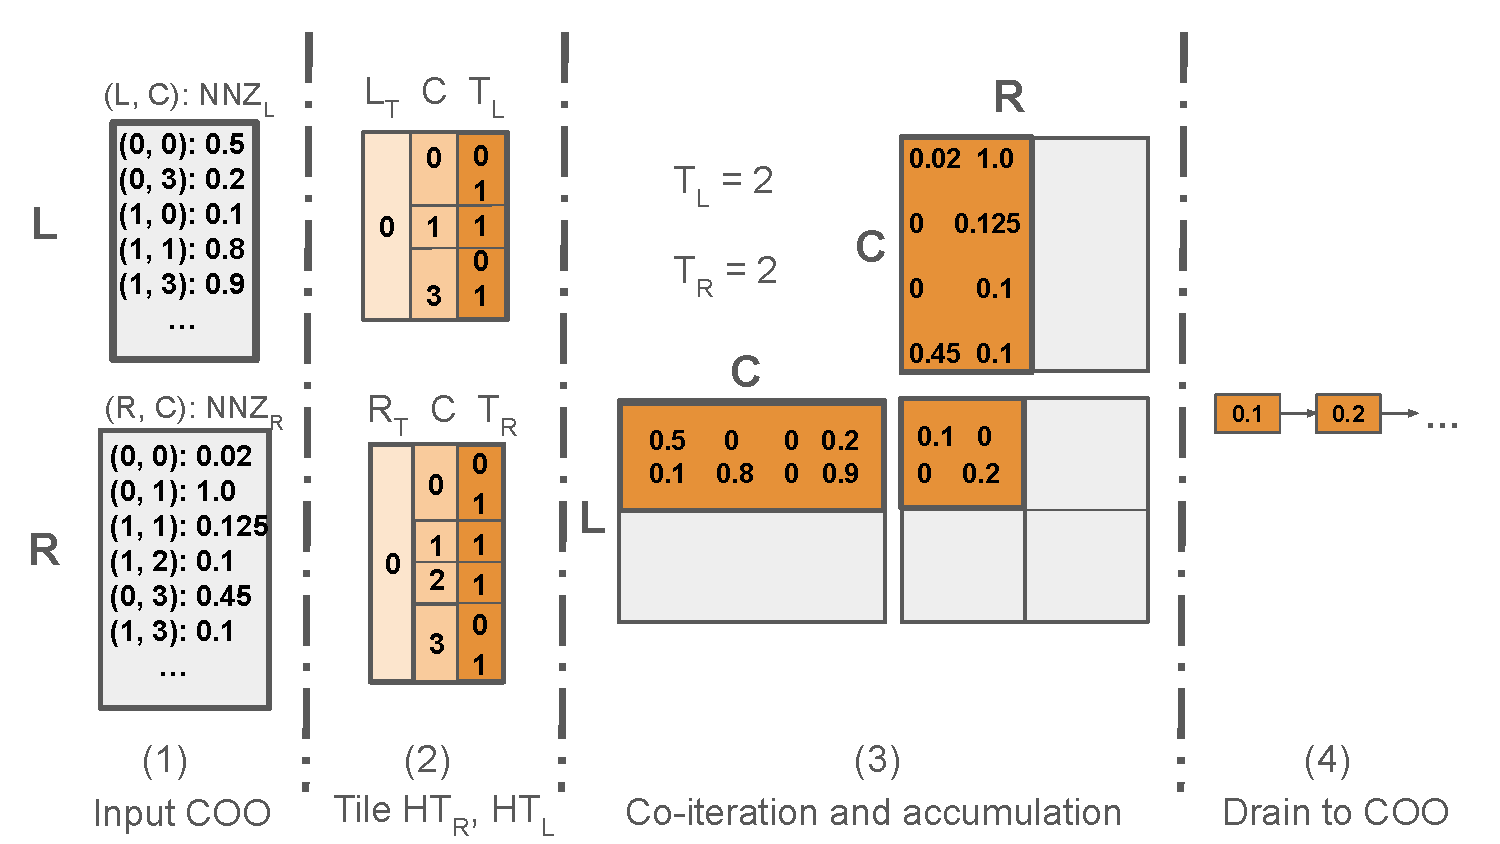
\includegraphics[scale=0.35]{fastcc system diag.pdf}
\caption{Intermediate steps of the FaSTCC contraction.}
\label{fig:frostt}
\end{figure}
% {\color{red} \bf We are no longer just Tiled CO; we have unified with CI; presentation of the algorithmic details need adaptation to match teh generalization.}
% The CO scheme described earlier (Algorithm~\ref{algo:co}) uses a 2D workspace $\mathit{WS}$ indexed by $l\in \mathbb{L}$ and $r\in \mathbb{R}$. Each workspace element 
% $\mathit{WS}(l,r)$ accumulates a series of contributions to output element $\mathit{Out}(l,r)$. 

In this section we present \ourtool, an efficient parallel implementation of a 2D-tiled CO scheme for sparse tensor contractions. As introduced in the previous section, the $\mathbb{L} \times \mathbb{R}$  index space of the output tensor is partitioned into ${\mathit{NL} \ast \mathit{NR}}$ tiles, where $\mathit{NL} = \lceil|\mathbb{L}| / \mathit{T_L} \rceil$ and $\mathit{NR} = \lceil|\mathbb{R}| / \mathit{T_R} \rceil$.

\subsection{Tiling and Workspace Design}
%\pp{We need a figure caption.}
%A key feature of our approach is that we define 2D tiling of index space $\mathbb{L} \times \mathbb{R}$ and use a workspace $\mathit{WS}$ that accumulates only the elements of that data tile of $\mathit{Out}$.
%This approach has two advantages. First, without tiling, the amount of memory needed for the workspace may become prohibitive. Second, tiling allows for improved data locality. 
%Both advantages are elaborated later in the paper and are illustrated with experimental studies [TODO: add discussion later]. 

%The tiling approach is parameterized by tile sizes $\mathit{TL}$ and $\mathit{TR}$.
%Later we discuss the considerations for choosing these tile sizes.
%For simplicity of presentation, we assume that $|\mathbb{L}|$ is a multiple of $\mathit{TL}$ (and similarly for $\mathit{TR}$). The handling of the general case with partial tiles is straightforward and not discussed due to space constraints. Let $\mathit{NL} = |\mathbb{L}| / \mathit{TL} $ and $\mathit{NR} = |\mathbb{R}| / \mathit{RL} $. 

\paragraph{Output tiles and input tiles}
Consider an output data tile $\mathit{Out}_{i,j}$ where $0\le i < \mathit{NL}$ and $0\le j < \mathit{NR}$. The tile is indexed by intra-tile indices $l$ and $r$ such that $0 \le l < \mathit{T_L}$ and $0 \le r < \mathit{T_R}$. Element $\mathit{Out}_{i,j}(l,r)$ corresponds to 
$\mathit{Out}(i\ast \mathit{T_L}+l,j \ast \mathit{T_R} + r)$. 

%[TODO: add a figure] 
To compute $\mathit{Out}_{i,j}$, we need a 1D tile $L_i$ of the left tensor $L$ and a 1D tile $R_j$ of the right tensor $R$. Here $L_i$ corresponds to elements $L(c,l)$ such that $i\ast \mathit{T_L} \le l < (i+1) \ast \mathit{T_L}$. Similarly, $R_j$ corresponds to elements $R(c,r)$ such that $j\ast \mathit{T_R} \le r < (j+1) \ast \mathit{T_R}$. To reflect this tiling of the inputs,
we represent the left input tensor using $\mathit{NL}$ hash tables of the form 
$$\mathit{HL}_i: \mathbb{C} \rightarrow \mathcal{P}(\{ 0, \ldots, \mathit{T_L} -1\} \times \mathbb{V})$$ 
and the right input tensor using $\mathit{NR}$ hash tables of the form 
$$\mathit{HR}_j: \mathbb{C} \rightarrow \mathcal{P}(\{ 0, \ldots, \mathit{T_R} -1\} \times \mathbb{V})$$ 
Map $\mathit{HL}_i$ represents input tile $L_i$ while $\mathit{HR}_j$ represents input tile $R_j$. The maps store intra-tile indices for the non-contraction data dimensions, together with the corresponding non-zero data values. For example, each $\langle l,\mathit{lv} \rangle \in \mathit{HL}_i(c)$ corresponds to an input element $L(c,i\ast \mathit{T_L}+l)$ with value $\mathit{lv}$. 

\paragraph{\ourtool \ algorithm} At the outermost level, Algorithm~\ref{algo:fastcc} iterates over output tiles $\mathit{Out}_{i,j}$. 
%Note that this iteration can be done in parallel, as discussed later [TODO: add discussion later]. 
For every $c$ such that both 
$\mathit{HL}_i$ and $\mathit{HR}_j$ contain some non-zero elements for $c$, the workspace $\mathit{WS}$ accumulates the contributions to $\mathit{Out}_{i,j}$ due to $c$. The output tile is then ``drained'' to the output tensor, with appropriate remapping of intra-tile indices $l$ and $r$. 
%This draining can also zero out the corresponding workspace elements, in preparation for the next iteration of the $j$ loop.

\begin{algorithm}[h]
\DontPrintSemicolon
\LinesNumbered
\For{$i \gets 0$ \KwTo $\mathit{NL} - 1$}{
\For{$j \gets 0$ \KwTo $\mathit{NR} - 1$}{
$\mathit{WS} \gets \emptyset$ \;
\For{$c \in \mathit{HL}_i.\mathit{keys}$}{
\If{$c \in \mathit{HR}_j.\mathit{keys}$}{
  \For{$\langle l,\mathit{lv} \rangle \in \mathit{HL}_i(c)$}{
    \For{$\langle r,\mathit{rv} \rangle \in \mathit{HR}_j(c)$}{ 
        $\mathit{WS}.\mathit{upsert}(l,r,\mathit{lv} \ast \mathit{rv})$ \;
}
}
}
}
\For{$\langle l, r \rangle \in \mathit{WS}.\mathit{keys}$}{
$\mathit{Out}.\mathit{append}(i\ast \mathit{T_L}+l,j \ast \mathit{T_R} + r, \mathit{WS}(l,r))$
}
% OLD VERSION
%\For{$c \in \mathbb{C}$}{
%  $\mathit{WS} \gets \emptyset$ \;
%  \For{$\langle l,\mathit{lv} \rangle \in \mathit{HL}_i(c)$}{
%    \For{$\langle r,\mathit{rv} \rangle \in \mathit{HR}_j(c)$}{ 
%        $\mathit{WS}.\mathit{upsert}(l,r,\mathit{lv} \ast \mathit{rv})$ \; } }
%          \For{$\langle l, r \rangle \in \mathit{WS}.\mathit{keys}$}{
%    $\mathit{Out}.\mathit{append}(l, r, \mathit{WS}(l,r))$ } }
    }}
\caption{\ourtool\ contraction\label{algo:fastcc}}
\end{algorithm}


\subsection{Implementation Details and Parallelization Techniques}
The \ourtool\ contraction has four steps: (1) construction of maps $\mathit{HL}_i$ and $\mathit{HR}_j$, (2) iteration over matching positions of $\mathit{HL}_i$ and $\mathit{HR}_j$,  (3) accumulation of partial results in the workspace, and (4) draining the workspace into the output COO list. Next we describe the parallel implementation of each of these steps individually.


\paragraph{Parallel construction of hash tables} Recall that non-zero elements of the left operand tensor $L$
are represented via hash tables $\mathit{HL}_i : \mathbb{C} \rightarrow \mathcal{P}(\{ 0, \ldots, \mathit{T_L} -1\} \times \mathbb{V})$. 
Each element $L(l, c)$ with value $\mathit{lv}$ is represented in map $\mathit{HL}_i$, where $i = \left \lfloor{l/\mathit{T_L}} \right \rfloor$, such that set $\mathit{HL}_i(c)$ contains a pair with the intra-tile index (e.g., $l\bmod \mathit{T_L}$) and the value $\mathit{lv}$. The representation of the right operand $R$ is similar.
This is illustrated in Figure~\ref{fig:frostt}, step 2 (tile hash tables). The example shows the computation of one output tile.
%In the example the number of tiles, $T_L = T_R = 2$. Only tile $L_T = R_T = 0$ is shown. $L$ from the original tensor maps directly to $T_L$.

Construction of these hash tables is performed in parallel.
Half the threads work on $\mathit{HL}$ while the other half works on $\mathit{HR}$.
This is implemented using OpenMP parallel regions with nested parallelism.
Each thread in the left team reads the input tensor $L$ in parallel, adding any points that are inside the thread's tile spaces to thread-local hash tables.
For example, thread $0$ in the left team is responsible for constructing all $\mathit{HL}_i$ with $i \bmod \mathit{num\_threads} = 0$, thread $1$ builds all $\mathit{HL}_i$ with $i \bmod \mathit{num\_threads} = 1$, and so on. 

\paragraph{Parallel co-iteration over $\mathit{HL}_i$ and $\mathit{HL}_j$}
We parallelize the co-iteration using a task queue.
Each tile-tile contraction (i.e., each combination of $i$ and $j$ values that computes some output tile $\mathit{Out}_{i,j}$ in Algorithm~\ref{algo:fastcc}) is defined as a separate task. These tasks are embarrassingly parallel, as each tile from the inputs is read-only, and each pair of input tiles \{$i$, $j$\} uniquely writes one tile of output.
Furthermore, since tasks are mapped to threads at run time, load imbalance is much lower than it would have been if we partitioned the index space of the non-zero elements. We use Taskflow for implementing this task queue \cite{taskflow}.


\paragraph{Parallel accumulation of partial results}
The result of this contraction is accumulated into a thread-local tile $\mathit{WS}_t$.
Based on an approach described later in Section~\ref{sec:model}, this can either be dense or sparse workspace.
At the end of the accumulation, $\mathit{WS}_t$ is drained into a thread-local COO linked list.

A dense tile structure includes:
(1) a buffer $\mathit{nnz}$ of size $\mathit{T_L} \ast \mathit{T_R} $ to hold non-zero elements of the tile, (2) a buffer 
$\mathit{apos}$ of the same size to hold integers corresponding to the active positions in the tile, and 
(3) a bitmask $\mathit{bm}$ with $\frac{\mathit{T_L} \ast \mathit{T_R}}{8}$ bits.
An update at position $p$ to this tile performs the following operations:
\begin{enumerate}
    \item Test and set bit $p$ of bitmask $\mathit{bm}$
    \item If the initial value of $\mathit{bm[p]}$ was $0$, append $\mathit{p}$ to $\mathit{apos}$
    \item Update the non-zero element at $\mathit{nnz[p]}$ with the new value
\end{enumerate}
The update operation takes constant time, and requires three random accesses to dense spaces.
In case the accumulator is sparse, we use an open addressed hash table and the update operation lowers to an upsert operation on the hash table, which is expected to execute in constant time.
This is shown in Figure~\ref{fig:frostt}, step 3, where the tile output data is computed from the input tile hash tables.

\paragraph{Parallel drain from tiles to COO output}
Once the tile has been filled with data,
the thread that owns that tile has to write the data to the COO list before working on the next tile.
In case the tile is a sparse accumulator, the thread simply iterates over the underlying hash table and appends to the COO list each non-zero with key as co-ordinate and value as the data.

For dense tiles, we use array $\mathit{apos}$ to perform the drain faster.
The thread iterates over this array of active non-zero positions within the tile.
It reads the non-zero elements from array $\mathit{nnz}$ with positions as given in $\mathit{apos}$, i.e. $\mathit{nnz[apos[iter]]}$, and appends them to the COO list.
Therefore, we iterate only over the non-zeros instead of iterating over the entire dense tile area of size $\mathit{T_L} \ast \mathit{T_R}$.
This is shown in Figure \ref{fig:frostt}, step 4 (drain to output COO) where the non-zeros from the tile are extracted and stored in the COO linked list.

\paragraph{COO representation for the output}
With the above four steps, we construct one COO list per thread that represents disjoint sets of the sparse tensor data.
The master thread concatenates these disjoint thread-local lists
using pointer movements (no data copies) into one output COO result.
We implement a memory pool layer to make the COO construction faster.
Each thread gets heap allocations in chunks of 512MB as it pushes non-zeros to the thread-local COO.
As the threads complete, they free up their local heap allocations.


%Recall from Algorithm~\ref{algo:tiled-co} that a workspace $\mathit{WS}$ is used to accumulate contributions to an output data tile $\mathit{Out}_{i,j}$ for each pair of values of outer iterators $i$ and $j$. We consider two approaches for 
%the design of this workspace. 

%When using a \emph{dense workspace}, a contiguous buffer with $\mathit{TL} \ast \mathit{TR}$ floating-point values can be used. For any $l$ and $r$, $\mathit{WS}.\mathit{upsert}(l,r,\mathit{lv} \ast \mathit{rv})$ updates the corresponding value in the buffer. In this case, the workspace should be zeroed out at the start of each iteration of the $j$ loop from Algorithm~\ref{algo:tiled-co}.
%This ``reset'' is performed at the end of the previous $j$ iteration: whenever a workspace element is appended to $\mathit{Out}$, it is immediately reset to a zero value. 
%[TODO: how do we know which elements of the dense workspace have been touched?]

%An alternative approach that reduces memory consumption is to implement $\mathit{WS}$ with a hash map; we refer to this 
%choice as a \emph{sparse workspace}. When the output data tiles are very sparse, a sparse workspace 
%can achieve significant memory savings. As a consequence, this makes it possible to increase the tile size significantly without running out of memory. In the next section, we discuss a performance modeling approach that further characterizes the trade-offs of these two choices, together with the considerations for selecting corresponding tile sizes. 

